\section{Segmentation}
The first step towards graph recognition is segmentation. This step identifies the segmentation points in the input graph. These points are fed into the recognition task to identify a component. Our implementation is based on the idea presented by \citeauthor{daly2015hand} \cite{daly2015hand} and assumes that the entire component is drawn in one stroke. However, drawing multiple components in the same stroke is acceptable for our implementation.\\

The segmentation points identify the transition from one component to the next. These are referred to as true segmentation points.  However, there are certain challenges in the segmentation task. These challenges arise from the fact that there might be additional points in a component with similar geometric properties as true segmentation points. This is shown in Figure \ref{fig:seg_false_neg}. The challenges can be divided into two buckets: false positives and false negatives. The points that are incorrectly identified as segmentation points contribute to false positives. These cases are less severe as they can be handled in the classification step. The points that are true segmentation points but are missed by the segmentation algorithm are false negatives. These cases are more severe as we cannot recover from these errors. The goal of the segmentation algorithm would be to minimize false positives while ensuring that there are no false negatives.\\

\begin{figure}
	\centering
	\begin{subfigure}{0.3\textwidth}
		\centering
		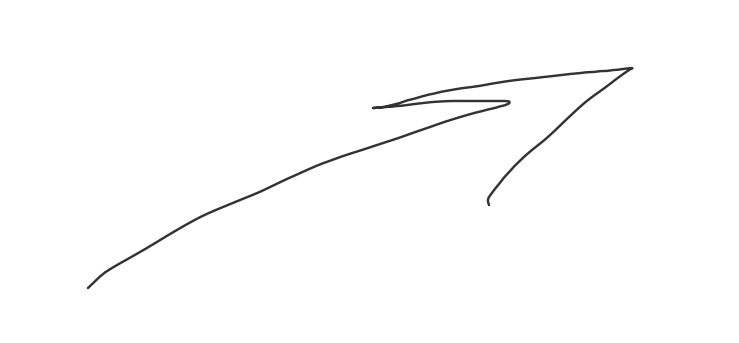
\includegraphics[scale=0.2]{./img/seg_orig.jpg}
	\end{subfigure}
	\begin{subfigure}{0.3\textwidth}
		\centering
		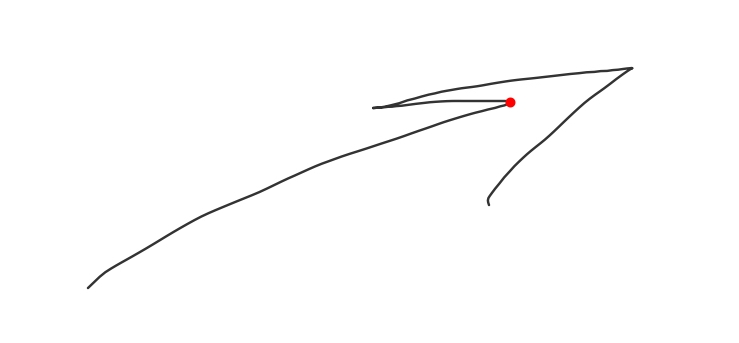
\includegraphics[scale=0.2]{./img/seg_true_seg.jpg}
	\end{subfigure}
	\begin{subfigure}{0.3\textwidth}j
		\centering
		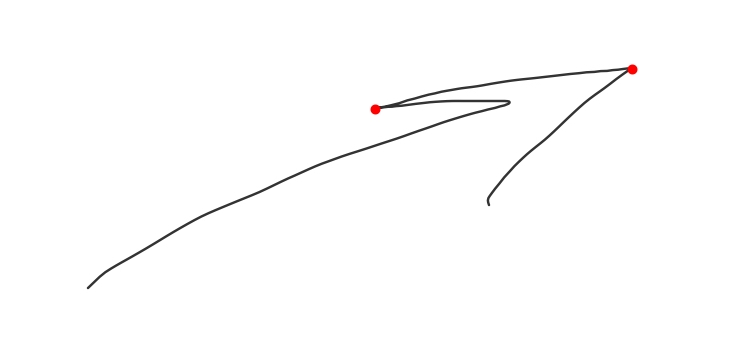
\includegraphics[scale=0.2]{./img/seg_false_seg.jpg}
	\end{subfigure}
	\caption{\textit{left} a line and arrow head drawn in one stroke, \textit{middle} true segmentation point, \textit{right} additional points with similar properties as true segmentation points}
	\label{fig:seg_false_neg}
\end{figure}

\subsection{Algorithm}
The algorithm to identify segmentation points is based on the observation that there are abrupt changes in curvature at these points. This is based on the properties of transition that can occur in the three types of graph components. This is shown in figure \ref{fig:seg_curvature}.\\

Before the curvature calculation, some pre-processing of input data is required. We use iPyCanvas \cite{ipycanvas} to capture the coordinates of the drawn components. The number of coordinates captured depends on the drawing speed. If the drawing speed is higher in certain regions, the number of points captured will be higher in those region. This count is normalized by considering the distance between two points. If the Euclidean distance between two consecutive points, $P_i$ and $P_{i+1}$, is less than a threshold, $d_t$, we drop $P_{i+1}$. Here, $d_t$ is a hyperparameter which needs to be trained based on the input data. For our usecase, $d_t = 1$ works well.\\

The curvature of a point $P_i$ is computed by calculating the angles between vectors formed by joining $P_{i-s}$ and $P_i$ and $P_i$ and $P_{i+s}$. $s$ is the second hyperparameters. For our usecase, we have kept $s=3$ based on experiments.

\begin{equation}
	C_s(P_i) = \arccos \left(  \frac{\overrightarrow{P_{i-s} P_i} \cdot \overrightarrow{P_i P_{i+s}}}{ \Vert \overrightarrow{P_{i-s} P_i}  \Vert \; \Vert \overrightarrow{P_i P_{i+s}} \Vert  } \right) 
\end{equation} 

Once the curvature is computed for all captured points, we compute the abnormality. This metric is used in identifying the abrupt and significant changes in the curvature. The abnormality of a point $P_i$ is defined by how the curvature at that point differs from the average curvature of the surrounding points.
\begin{equation}
	A_{s,w}(P_i) = C_s(P_i) - \frac{\sum_{j=a}^{i-1} C_s(P_j) + \sum_{j=i+1}^{b} C_s(P_j)}{b - a}
\end{equation}
where $a = max(1, i-w)$ and $b = min(n, i+w)$.\\

$w$ is the third hyperparameter. For our usecase, we use $w=5$ based on our experiments. Next, we need to find ranges of points where $k A_{s, w}(P_i) > 1$ and select the point with maximum abnormality in each range as the segmentation point. The multiplication factor $k$ is the fourth hyperparameter.\\

\begin{figure}
	\centering
	\begin{subfigure}{0.9\textwidth}
		\centering
		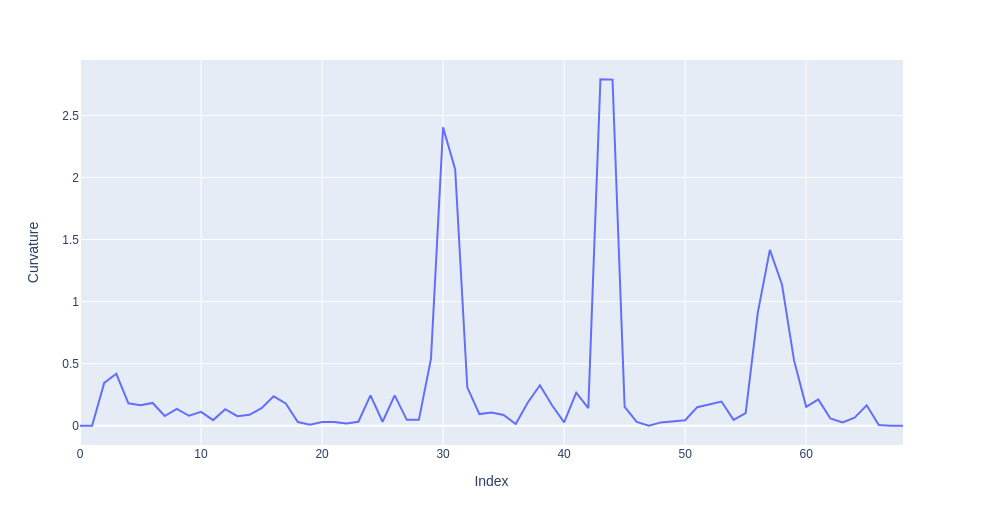
\includegraphics[scale=0.5]{./img/seg_curvature_plot}
	\end{subfigure}
	\caption{Curvature plot for the components shown in figure \ref{fig:seg_false_neg}. The peaks represent the segmentation points.}
	\label{fig:seg_curvature}
\end{figure}

\subsection{Experiments}
To test the segmentation algorithm, we drew some components and shapes manually on iPyCanvas and validated the results. These are shown in figure \ref{fig:seg_results}.
\begin{figure}
	\centering
	\begin{subfigure}{0.8\textwidth}
		\centering
		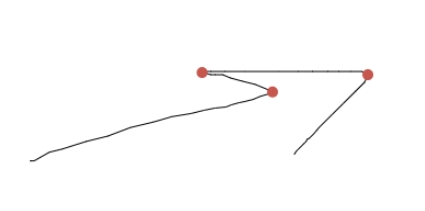
\includegraphics[scale=0.6]{./img/seg_results_arrow.jpg}
	\end{subfigure}
	\begin{subfigure}{0.8\textwidth}
		\centering
		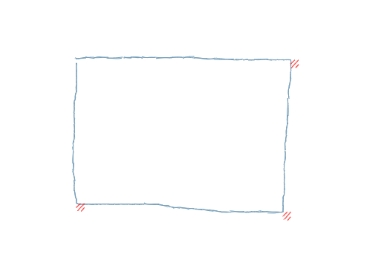
\includegraphics[scale=0.6]{./img/seg_results_rect.jpg}
	\end{subfigure}
	\begin{subfigure}{0.8\textwidth}
		\centering
		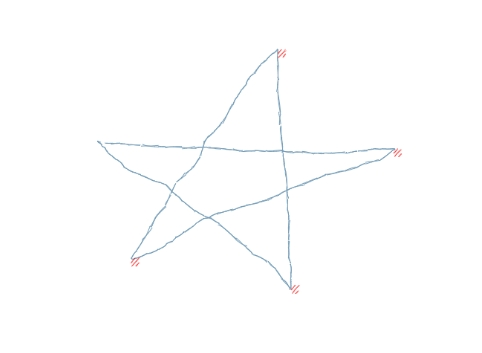
\includegraphics[scale=0.6]{./img/seg_results_pentagram.jpg}
	\end{subfigure}
	\caption{Detected segmentation points (highlighted in red).}
	\label{fig:seg_results}
\end{figure}

%\subsection{Future Work}
%The immediate next step is to integrate the segmentation module with the classification module and fine tune the four hyperparameters discussed in this section. In addition, we will work on extending the algorithm to support offline graph recognition.